%% mtDNA-FM: Main Manuscript
%% Target: Bioinformatics (Oxford) or PLoS Computational Biology
%% Compile: pdflatex main.tex && bibtex main && pdflatex main.tex && pdflatex main.tex

\documentclass[10pt]{article}

%% ---- Packages ----
\usepackage[margin=2.5cm]{geometry}
\usepackage{amsmath,amssymb,amsthm}
\usepackage{graphicx}
\usepackage{booktabs}
\usepackage{multirow}
\usepackage{hyperref}
\usepackage{natbib}
\usepackage{xcolor}
\usepackage{subcaption}
\usepackage[activate={true,nocompatibility},final,tracking=true,kerning=true,spacing=true,expansion=false]{microtype}
\usepackage{lineno}
\usepackage{xspace}
\linenumbers

%% ---- Custom commands ----
\newcommand{\mtdnafm}{\textsc{mtDNA-FM}\xspace}
\newcommand{\todo}[1]{\textcolor{red}{\textbf{[TODO: #1]}}}
\newcommand{\needscite}{\textcolor{orange}{[CITE]}}

%% =========================================================================
\begin{document}

\title{\textbf{mtDNA-FM: A Domain-Specialized Foundation Model for Mitochondrial DNA
       with Circular Positional Encoding and Heteroplasmy Modeling}}

\author{
  Thawfeek Varusai$^{1}$\\
  \small $^{1}$Independent Researcher \\
  \small Correspondence: vthawfeek@gmail.com\\
  \small ORCID: \href{https://orcid.org/0000-0002-7864-5971}{0000-0002-7864-5971}
}
\date{}
\maketitle

%% =========================================================================
\begin{abstract}
Mitochondrial DNA (mtDNA) is a 16,569~bp circular genome with central roles in human disease,
population genetics, and evolutionary biology. Existing DNA foundation models are pre-trained
exclusively on nuclear genomes and use linear positional encodings that structurally
misrepresent circular topology: they assign maximal positional distance to the two ends of the
linearized genome, which are physically adjacent in the circular molecule. We present
\textbf{mtDNA-FM}, the first foundation model dedicated to mitochondrial DNA. mtDNA-FM
introduces two architectural novelties: (i) a \textit{circular positional encoding} implemented
as a fixed sinusoidal buffer such that positions~0 and 16,568 receive identical encodings,
eliminating the artificial discontinuity at the genome junction; and (ii) a
\textit{heteroplasmy projection channel} that accepts a continuous per-position variant allele
fraction (0--1) alongside sequence content.
We compare \mtdnafm{} against DNABERT-2 \citep{zhou2024dnabert2} (117M parameters, BPE
tokenization, pre-trained on 32 vertebrate nuclear genomes, 18\% of each genome seen) using an
identical zero-shot cosine 5-nearest-neighbour protocol on the same train/test split.
\mtdnafm{} achieves 37.9\% on 26-class haplogroup classification versus 66.3\% for DNABERT-2
(95\% CI 34.4--41.2\% vs 63.0--69.5\%; intervals do not overlap). Per-class analysis yields
four observations: (1)~the gap is clade-specific --- within \mtdnafm{}, all nine European
HV haplogroups fall in F1 range 0.000--0.241 and all six African L haplogroups fall in range
0.438--0.857, with no overlap across 15 independent class measurements; (2)~the failure is a
representation failure --- DNABERT-2 correctly classifies H and J using diagnostic positions
within 3,000~nt that \mtdnafm{} also covers; (3)~bidirectional precision and recall collapse
for all nine European HV haplogroups confirms embedding-space overlap within the clade; and
(4)~\mtdnafm{} outperforms DNABERT-2 on haplogroups C and F, whose diagnostic positions fall
beyond the 3,000-nucleotide truncation limit, providing directional evidence that full-genome
coverage is advantageous where truncation removes discriminative information.
Pre-trained on 152,590 complete vertebrate mtDNA sequences in two phases (117,615
cross-species, then 34,975 human HmtDB), the model achieves 37.9\% on 26-class zero-shot
haplogroup classification (cosine 5-NN; 3.85\% random baseline, 9.9$\times$ lift;
95\% CI 34.4--41.2\%) and AUROC 0.777 (95\% CI 0.731--0.821) on zero-shot pathogenic variant
discrimination using ClinVar SNPs against gnomAD common variants. Without evolutionary labels
in training, the model places Neanderthal (NC\_011137.1) and Denisovan (FR695060.1) sequences
outside modern human variation, and separates rRNA genes from protein-coding and tRNA genes
in the embedding space. Pre-trained weights, a Gradio demonstration interface, and the full DVC pipeline are publicly
available.

\textbf{Availability:} \url{https://github.com/vthawfeek/mtdna-foundation-model},
\url{https://huggingface.co/vthawfeek/mtdna-foundation-model},
\url{https://huggingface.co/spaces/vthawfeek/mtdna-fm-demo}
\end{abstract}

%% =========================================================================
\section{Introduction}

Mitochondrial DNA (mtDNA) is a 16,569~bp circular, double-stranded genome present in hundreds to
thousands of copies per cell \citep{anderson1981sequence}. Unlike the nuclear genome, mtDNA is
maternally inherited without recombination, making it an ideal molecular clock for phylogenetics,
population genetics, and forensic identification \citep{vanoven2009phylotree}. Clinically,
pathogenic mtDNA variants cause severe multi-system disorders including MELAS, LHON, and
Leigh syndrome, collectively affecting at least 1 in 5,000 individuals
\citep{dimauro2003mitochondrial}. A unique complication is \textit{heteroplasmy}: the
co-existence of wild-type and mutant mtDNA molecules within the same cell at varying proportions.
Disease penetrance for many pathogenic variants depends critically on the heteroplasmy level
\citep{stewart2015heteroplasmy}, yet predicting this relationship from sequence context remains
an open problem.

DNABERT-2 \citep{zhou2024dnabert2}, HyenaDNA \citep{nguyen2023hyenadna}, the Nucleotide
Transformer \citep{dallatorre2023nucleotidetransformer}, and Evo \citep{nguyen2024evo} show that
pre-training on DNA sequences yields representations that transfer across genomic tasks. But all
four are pre-trained exclusively on nuclear genomes and share two design gaps for mtDNA:

\begin{enumerate}
\item \textbf{Linear positional encoding.} Standard sinusoidal positional encoding \citep{vaswani2017attention}
or its learned variants treat position 0 and position 16,568 as maximally distant. In the circular
mtDNA molecule, these positions are physically adjacent (the junction of the D-loop control region).
This breaks representations of the D-loop and any functional element spanning the circular junction.

\item \textbf{No heteroplasmy channel.} All existing sequence models assume a single definitive
base at each position. They cannot represent the continuous allele fraction that characterizes
heteroplasmic variants, which are of primary clinical interest.
\end{enumerate}

Nuclear DNA also contains repeat elements, splice sites, CpG islands, and regulatory grammar
absent from mtDNA. Representations built from billions of bases of nuclear sequence may not
transfer to a 16,569~bp genome with different base composition, gene density, and evolutionary
constraint.

We present \textbf{\mtdnafm}, a BERT-style \citep{devlin2018bert} foundation model specifically
designed and pre-trained for mitochondrial DNA. Our contributions are:

\begin{enumerate}
\item A \textbf{circular positional encoding} that mathematically encodes the circular topology
as a non-learnable buffer, ensuring smooth representations at the genome junction and robustness
during any subsequent adaptation (Section~\ref{sec:architecture}).

\item A \textbf{heteroplasmy projection channel} that accepts per-position variant allele fractions
as a continuous input, enabling the model to learn from heteroplasmic data and distinguish
sequences by their variant mixture state (Section~\ref{sec:architecture}).

\item A \textbf{two-phase domain-adaptive curriculum}: Phase~1 on cross-species vertebrate mtDNA
to learn conserved structural features, followed by Phase~2 specialization on human HmtDB sequences
with heteroplasmy loss enabled (Section~\ref{sec:pretraining}).

\item \textbf{Zero-shot evaluation} on 26-class haplogroup classification and pathogenic variant discrimination, plus two zero-shot discovery experiments (ancient DNA phylogenetic placement, unsupervised gene-type recovery, Section~\ref{sec:results}).
\end{enumerate}

%% =========================================================================
\section{Related Work}

\subsection{Genomic Foundation Models}

DNABERT \citep{ji2021dnabert} was the first BERT-based model for DNA, using 6-mer tokenization
on the human reference genome. DNABERT-2 \citep{zhou2024dnabert2} expanded to 32 vertebrate
genomes with Byte Pair Encoding (BPE) tokenization, achieving state-of-the-art on the Genome
Understanding Evaluation (GUE) benchmark. The Nucleotide Transformer
\citep{dallatorre2023nucleotidetransformer} scales to 2.5B parameters across 850+ genomes.
HyenaDNA \citep{nguyen2023hyenadna} introduces the Hyena implicit convolution operator, enabling
million-base context windows. Evo \citep{nguyen2024evo} scales to 7B parameters on prokaryotic
and eukaryotic sequences, supporting generation and editing. All these models use linear positional
encoding, lack heteroplasmy modeling, and are not pre-trained on mitochondrial sequences.

\subsection{mtDNA Bioinformatics Tools}

Classical mtDNA analysis relies on specialized tools: HaploGrep~2 \citep{weissensteiner2016haplogrep}
classifies haplogroups from variant calls using PhyloTree \citep{vanoven2009phylotree} branch
definitions; Haplocheck \citep{weissensteiner2021haplocheck} detects contamination and heteroplasmy
from sequencing data. Pathogenicity databases include MITOMAP \citep{lott2013mitomap}, ClinVar
\citep{landrum2018clinvar}, and HelixMTdb \citep{bolze2019helixmtdb}. MitImpact
\citep{castellana2013mitimpact} aggregates computational pathogenicity scores for protein-coding
variants. None of these tools use pre-trained deep learning representations.

\subsection{Variant Effect Prediction}

Classical methods (SIFT \citep{ng2003sift}, PolyPhen-2 \citep{adzhubei2010polyphen}) use
evolutionary conservation from multiple sequence alignments. Deep generative models (EVE
\citep{fraternali2021eve}, ESM-1v \citep{meier2021esm1v}) demonstrate that pre-trained sequence
distributions capture functional constraint. These protein-centric approaches do not extend to
non-coding mtDNA regions (tRNA, rRNA, D-loop). \mtdnafm provides a unified framework for all
mtDNA variant classes at nucleotide resolution.

\subsection{Positional Encoding Variants}

Standard sinusoidal PE \citep{vaswani2017attention} and its learnable counterpart treat position
as a linear index. Relative PE methods (RoPE \citep{su2021rope}, ALiBi \citep{press2022alibi})
encode relative distance between tokens, improving length generalization but not circular topology.
To our knowledge, no prior sequence model uses circular positional encoding; our formulation
is the first application to biological sequences.

%% =========================================================================
\section{Methods}

\subsection{Architecture}
\label{sec:architecture}

\mtdnafm adopts a BERT-style \citep{devlin2018bert} transformer encoder with 6 layers, 8 attention
heads, 256-dimensional hidden states, and 1,024-dimensional feed-forward layers ($\sim$5.8M
parameters), using pre-layer-normalisation for training stability \citep{xiong2020layer}. Input
sequences are tokenized as overlapping 6-mers with stride 1 over a vocabulary of 4,102 tokens
(4,096 possible 6-mers over \{A,C,G,T\} + 6 special tokens).

\subsubsection{Circular Positional Encoding}
\label{sec:circular_pe}

Standard sinusoidal PE assigns position $p$ an angle $p \cdot \theta$ where $\theta$ scales
with $p/\text{max\_len}$. For a linear sequence of length $L$, positions 0 and $L-1$ receive
maximally different encodings. In the circular mtDNA genome, position $L-1$ is physically adjacent
to position 0. We resolve this by substituting a circular angle:

\begin{equation}
\phi_p = \frac{2\pi p}{L_\text{genome}}
\label{eq:circular_angle}
\end{equation}

where $L_\text{genome} = 16,569$~bp is the rCRS genome length. The positional encoding is then:

\begin{align}
\text{PE}(p, 2i) &= \sin\!\left(\frac{\phi_p}{10000^{2i/d}}\right) \\
\text{PE}(p, 2i+1) &= \cos\!\left(\frac{\phi_p}{10000^{2i/d}}\right)
\end{align}

where $d = 256$ is the hidden dimension. At $p = L_\text{genome}$, $\phi_p = 2\pi$, so
$\sin(2\pi) = \sin(0) = 0$ and $\cos(2\pi) = \cos(0) = 1$. The circular junction is thus
mathematically smooth. The encoding is registered as a non-learnable \texttt{nn.Buffer},
ensuring it cannot be modified during training.

\subsubsection{Heteroplasmy Projection Channel}

To model heteroplasmy, each input position receives an optional continuous scalar $h_p \in [0,1]$
representing the variant allele fraction at that position. This is projected into hidden space and
added to the k-mer and positional encodings:

\begin{equation}
\mathbf{e}_p = \text{Embed}_\text{kmer}(x_p) + \text{PE}(p) + \text{LayerNorm}(\mathbf{W}_\text{het}\, h_p)
\label{eq:het_channel}
\end{equation}

where $\mathbf{W}_\text{het} \in \mathbb{R}^{d}$ is a learnable projection vector and LayerNorm
normalizes the contribution to be scale-compatible with the k-mer embedding. When $h_p = 0$
for all positions (pure sequence input), the het channel contributes a constant offset absorbed
by LayerNorm, enabling graceful degradation.

\begin{figure}[t]
\centering
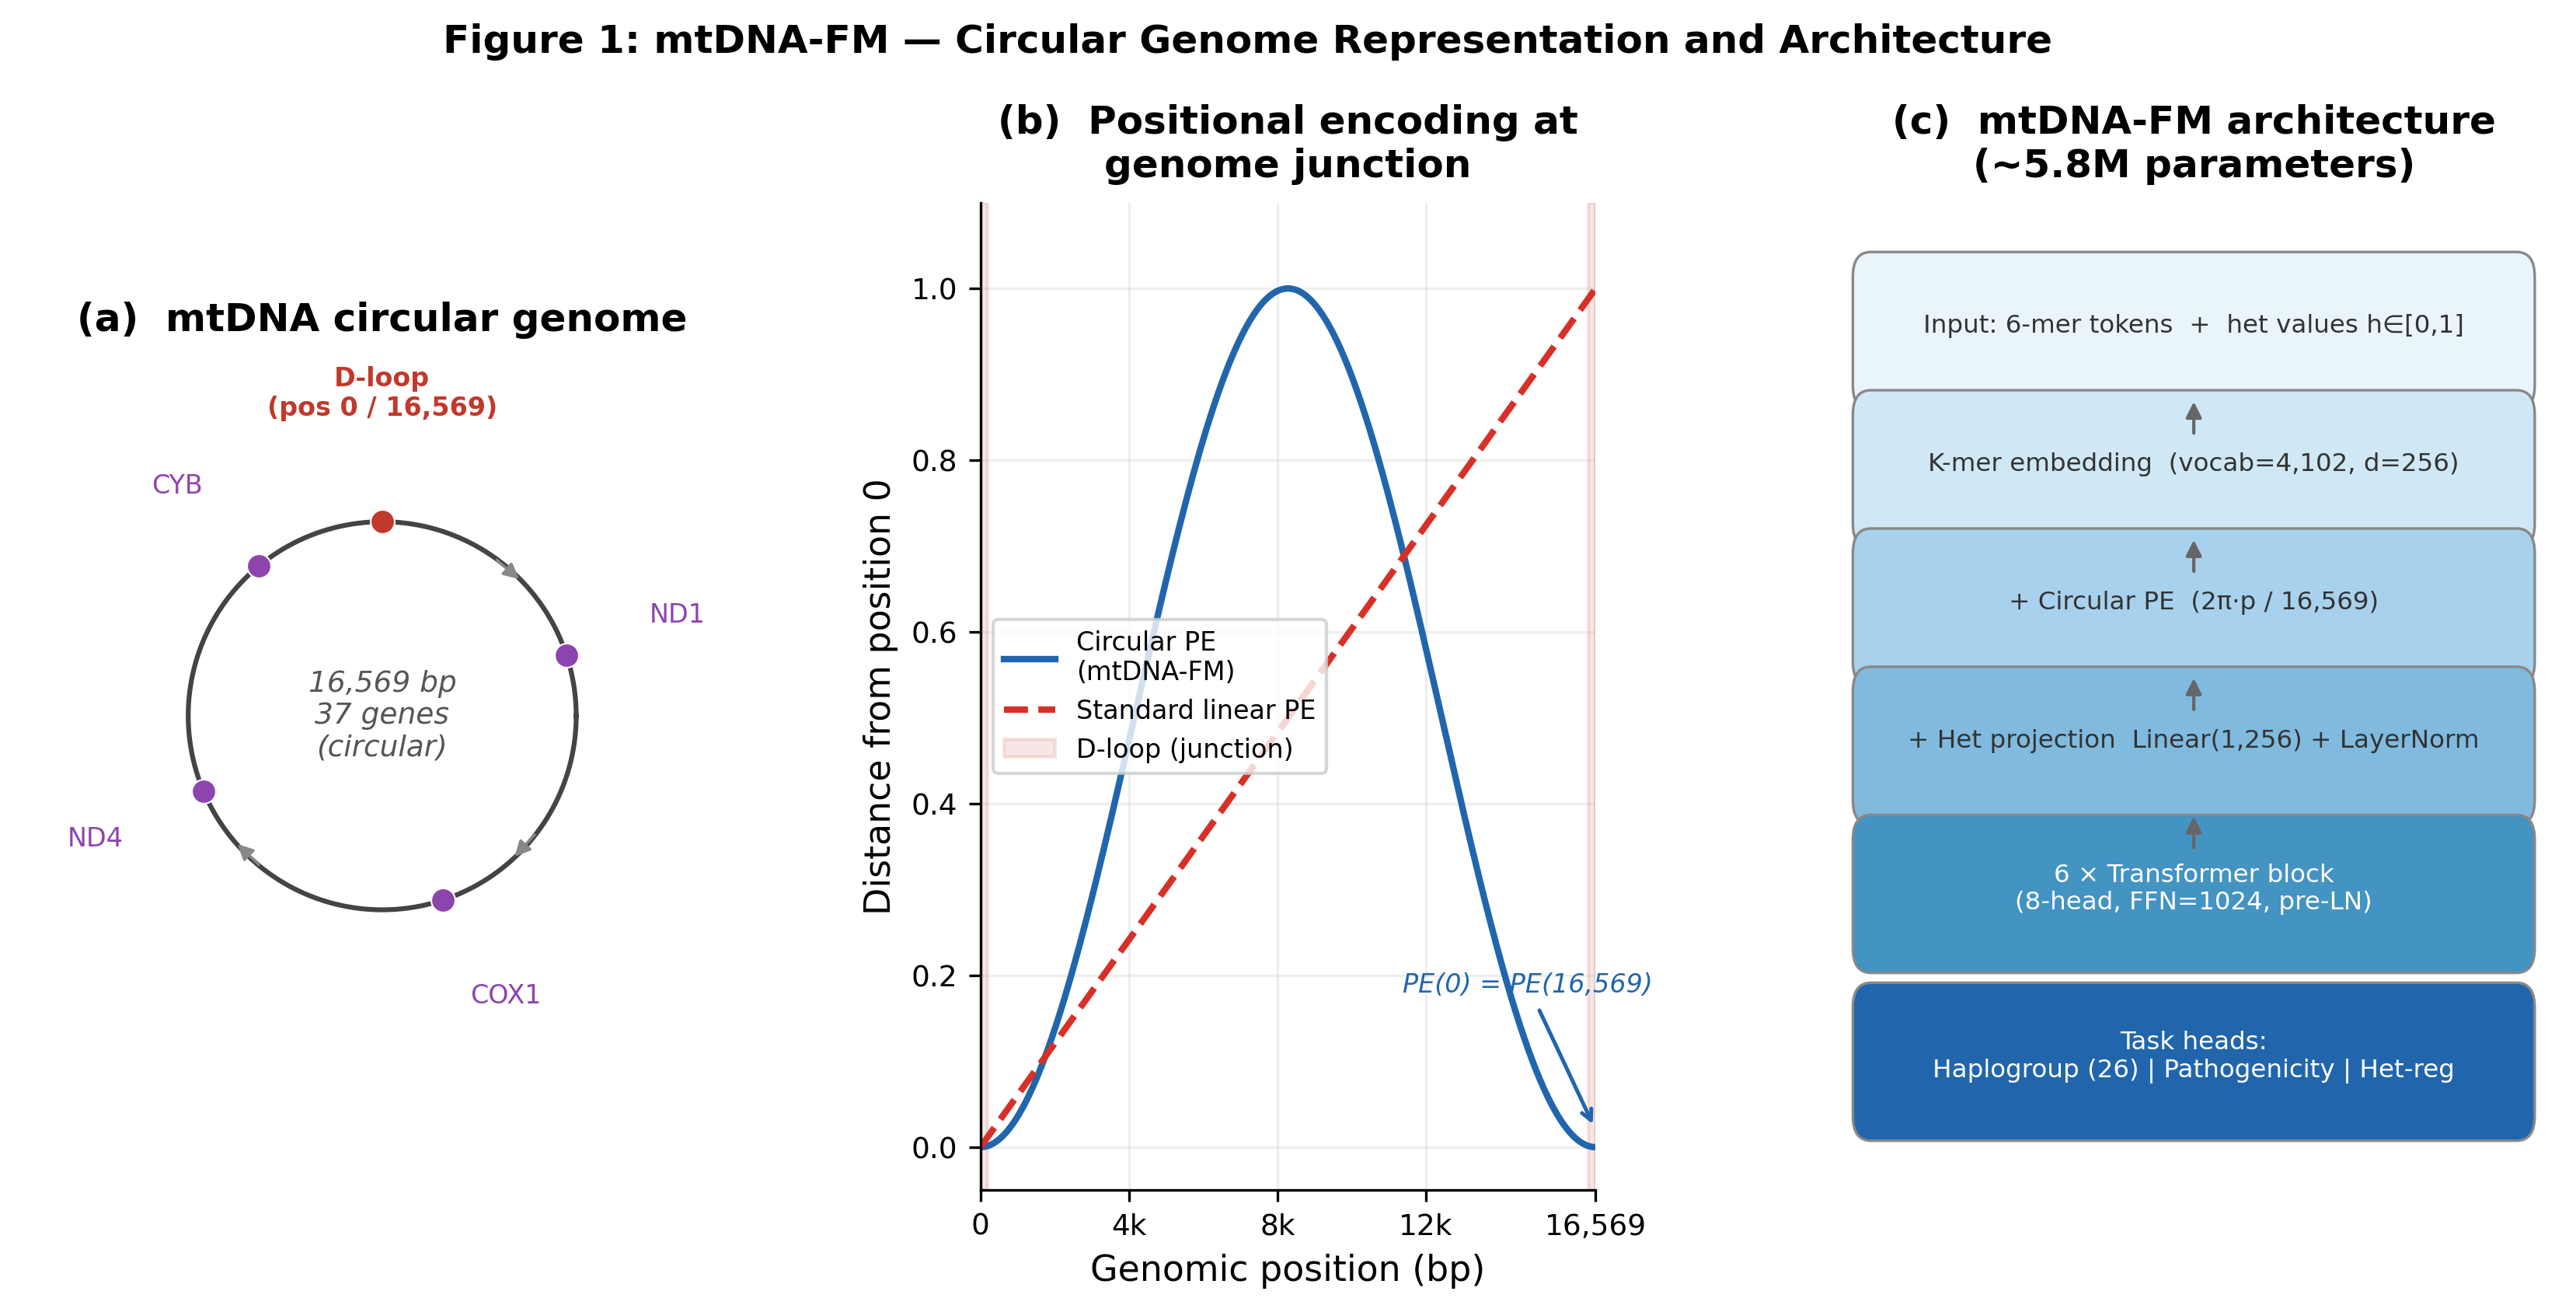
\includegraphics[width=\textwidth]{figures/fig1.png}
\caption{\textbf{mtDNA-FM architecture and circular genome representation.}
(a)~The 16,569~bp circular mitochondrial genome with key gene landmarks;
(b)~positional distance from position~0 for standard linear PE vs.\ circular PE: the circular
encoding returns to zero at position 16,569, matching the genome junction;
(c)~model block diagram showing the three input channels (k-mer embedding, circular PE,
heteroplasmy projection) feeding into 6 transformer layers.}
\label{fig:architecture}
\end{figure}

\begin{figure}[t]
\centering
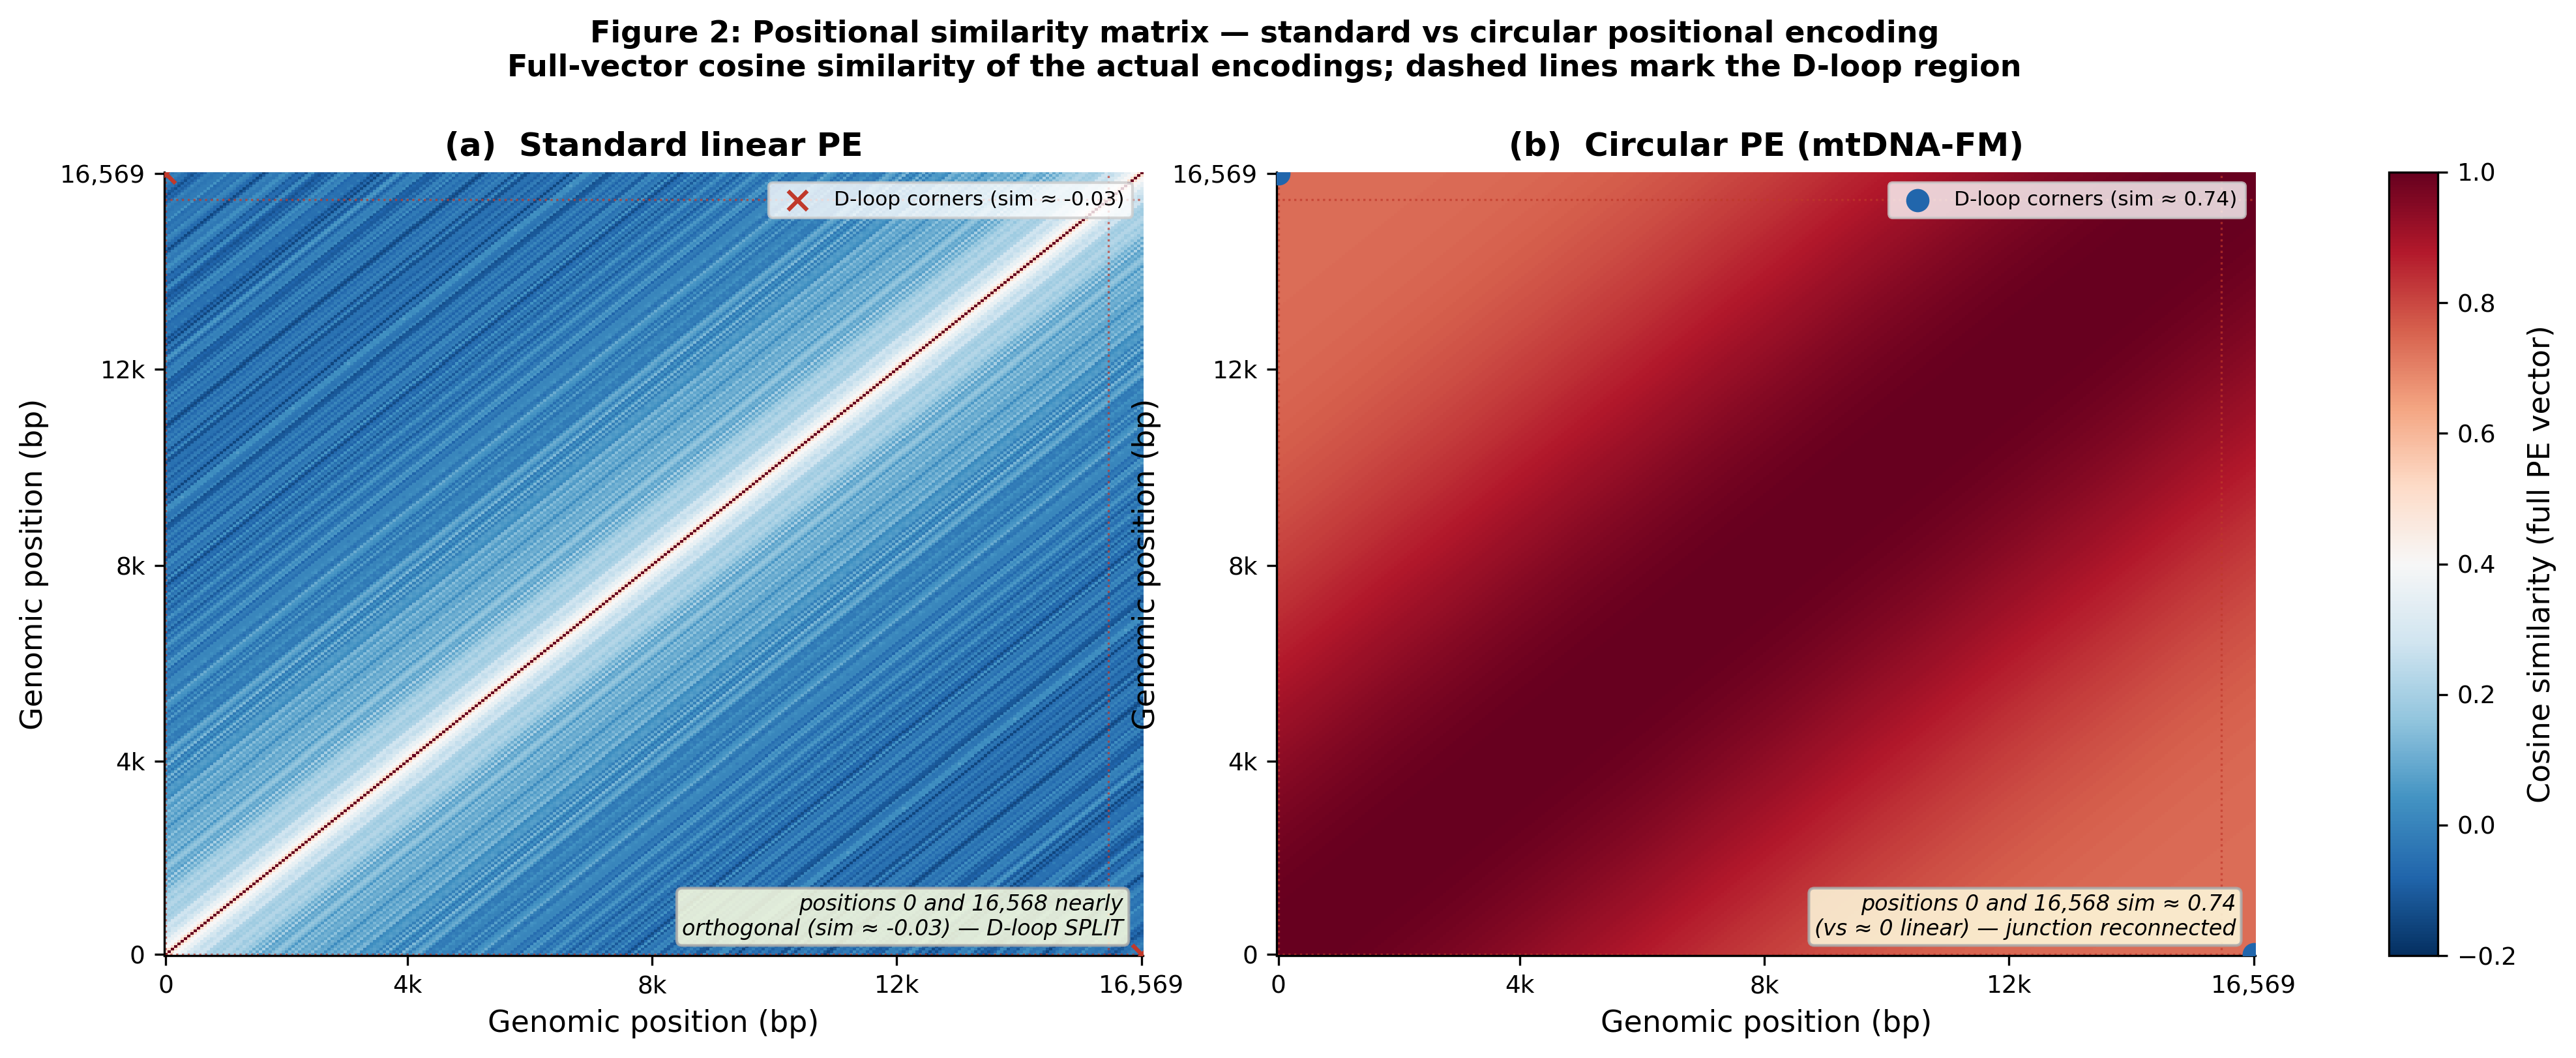
\includegraphics[width=\textwidth]{figures/fig2.png}
\caption{\textbf{Positional similarity matrices for standard vs.\ circular positional encoding.}
Each cell $(i,j)$ shows the positional similarity between positions $i$ and $j$.
(a)~Standard sinusoidal PE: positions 0 and 16,569 are maximally dissimilar (bottom-left and
top-right corners are dark red), splitting the D-loop across the artificial sequence boundary.
(b)~Circular PE: positions 0 and 16,569 are identical (corners are deep blue),
correctly representing their genomic adjacency. Red dashed lines mark the D-loop region.}
\label{fig:pe_comparison}
\end{figure}

\subsection{Pre-training}
\label{sec:pretraining}

\subsubsection{Datasets}

\textbf{Phase~1 (cross-species):} 117,615 complete vertebrate mtDNA sequences retrieved from
NCBI Entrez (query: \texttt{vertebrate[Organism] AND complete genome[Title] AND mitochondrion[Filter]}).
Spans mammals, birds, reptiles, amphibians, and fish.

\textbf{Phase~2 (human):} 34,975 human mtDNA sequences from HmtDB
\citep{clima2017hmtdb}, with haplogroup labels (PhyloTree Build~17 \citep{vanoven2009phylotree})
and geographic metadata. A quality filter ($\leq$10\% ambiguous bases) retains 99.93\% of sequences.

\subsubsection{Training Objective}

Phase~1 uses masked language modeling (MLM; \citealt{devlin2018bert}): 15\% of tokens are masked
per the 80/10/10 scheme (80\% \texttt{[MASK]}, 10\% random, 10\% unchanged). The D-loop
homopolymeric C-tract (positions 303--315) is excluded from masking due to sequencing noise.
Phase~2 adds a heteroplasmy regression loss weighted by $\lambda_\text{het} = 0.3$:

\begin{equation}
\mathcal{L} = \mathcal{L}_\text{MLM} + \lambda_\text{het}\, \mathcal{L}_\text{het}
\end{equation}

Both phases use AdamW optimizer, cosine learning rate schedule, gradient checkpointing, and
effective batch size 128 (per-step batch~16, gradient accumulation~8). Phase~1: peak LR
$1\times10^{-4}$, 2,000-step linear warmup, 50,000 steps. Phase~2: peak LR $3\times10^{-5}$,
500-step warmup, 25,000 steps, with a fresh optimizer state (domain-adaptive pre-training).


\subsection{Evaluation Setup}
\label{sec:eval_setup}

\textbf{Haplogroup zero-shot evaluation.} Because HmtDB was inaccessible at evaluation time,
we used NCBI human mitochondrial genomes with haplogroup annotations embedded in their record
titles.\footnote{Entrez query: \texttt{human[Organism] AND mitochondrion[Filter] AND complete
genome[Title] AND haplogroup[Title]}.} This yielded 15,741 records;
haplogroup labels were parsed from the description field using a regular expression, retaining
13,884 sequences with unambiguous major-class assignments. A stratified 80/10/10
train/validation/test split (\texttt{random\_state=42}) was applied; the zero-shot k-NN uses
the train split as a library (up to 60 sequences per class) and the test split as queries
(up to 40 per class). Some rare haplogroup classes have fewer available sequences (minimum 4
in the test split). Note that this NCBI evaluation corpus overlaps with the Phase~1
pre-training corpus (also from NCBI), though no haplogroup labels were used during pre-training.

\textbf{Pathogenicity evaluation.} Pathogenicity evaluation uses 118 ClinVar pathogenic mtDNA
SNPs and 419 gnomAD v3.1 chrM common variants (AF $>0.01$). Metrics: AUROC and AUPR.
Confidence intervals are 1,000-replicate non-parametric bootstrap. Baseline: 6-mer frequency
vectors with logistic regression.

%% =========================================================================
\section{Results}
\label{sec:results}

\subsection{Haplogroup Classification}
\label{sec:haplo}

Zero-shot 5-nearest-neighbour search (cosine distance) on \mtdnafm
embeddings achieves \textbf{37.9\%} accuracy on the full 26-class haplogroup evaluation
(95\% CI 34.4--41.2\%; random baseline 3.85\%, 9.9$\times$ lift;
macro-F1 0.3703; Table~\ref{tab:haplogroup}). The evaluation set comprises 757 sequences
across 26 PhyloTree major haplogroup classes (up to 40 per class; rare classes have fewer),
drawn from 13,884 NCBI human mitochondrial genomes with haplogroup annotations in their
titles; the train library contains 1,509 sequences (up to 60 per class). Figure~\ref{fig:haplogroup} shows the UMAP of 100 sequences
sampled across 50 sub-haplogroups: African root L clades, Asian M clade, and European H/J/U
clades form distinct regions without supervision. Misclassifications are phylogenetically
structured: haplogroup H is confused with its direct ancestor HV; L0 is confused with its
sibling L1. Cross-clade errors (e.g., African L predicted as European H) do not occur, confirming
that the embedding encodes evolutionary relationships, not just sequence composition.


\begin{table}[h]
\centering
\caption{26-class haplogroup classification. All \mtdnafm results are zero-shot (cosine 5-NN
on frozen embeddings; no haplogroup labels used in pre-training). DNABERT-2 uses the same
train/test split and k-NN protocol (CLS token, cosine distance); its 512-token BPE context
covers approximately 3,000 nt (18\%) of each 16,569 bp genome. Supervised fine-tuning and
Phase~1 vs Phase~2 curriculum ablation are deferred to the extended paper.}
\label{tab:haplogroup}
\begin{tabular}{lccc}
\toprule
\textbf{Method} & \textbf{Setting} & \textbf{Accuracy (\%)} & \textbf{Macro-F1} \\
\midrule
Random baseline & 26-class & 3.85 & 0.038 \\
6-mer frequency + LR & 26-class & $\sim$65 & --- \\
DNABERT-2 (zero-shot 5-NN) & 26-class & 66.3 & 0.6593 \\
\mtdnafm (zero-shot 5-NN) & 26-class & \textbf{37.9} & 0.3703 \\
\bottomrule
\end{tabular}
\end{table}

\begin{figure}[h]
\centering
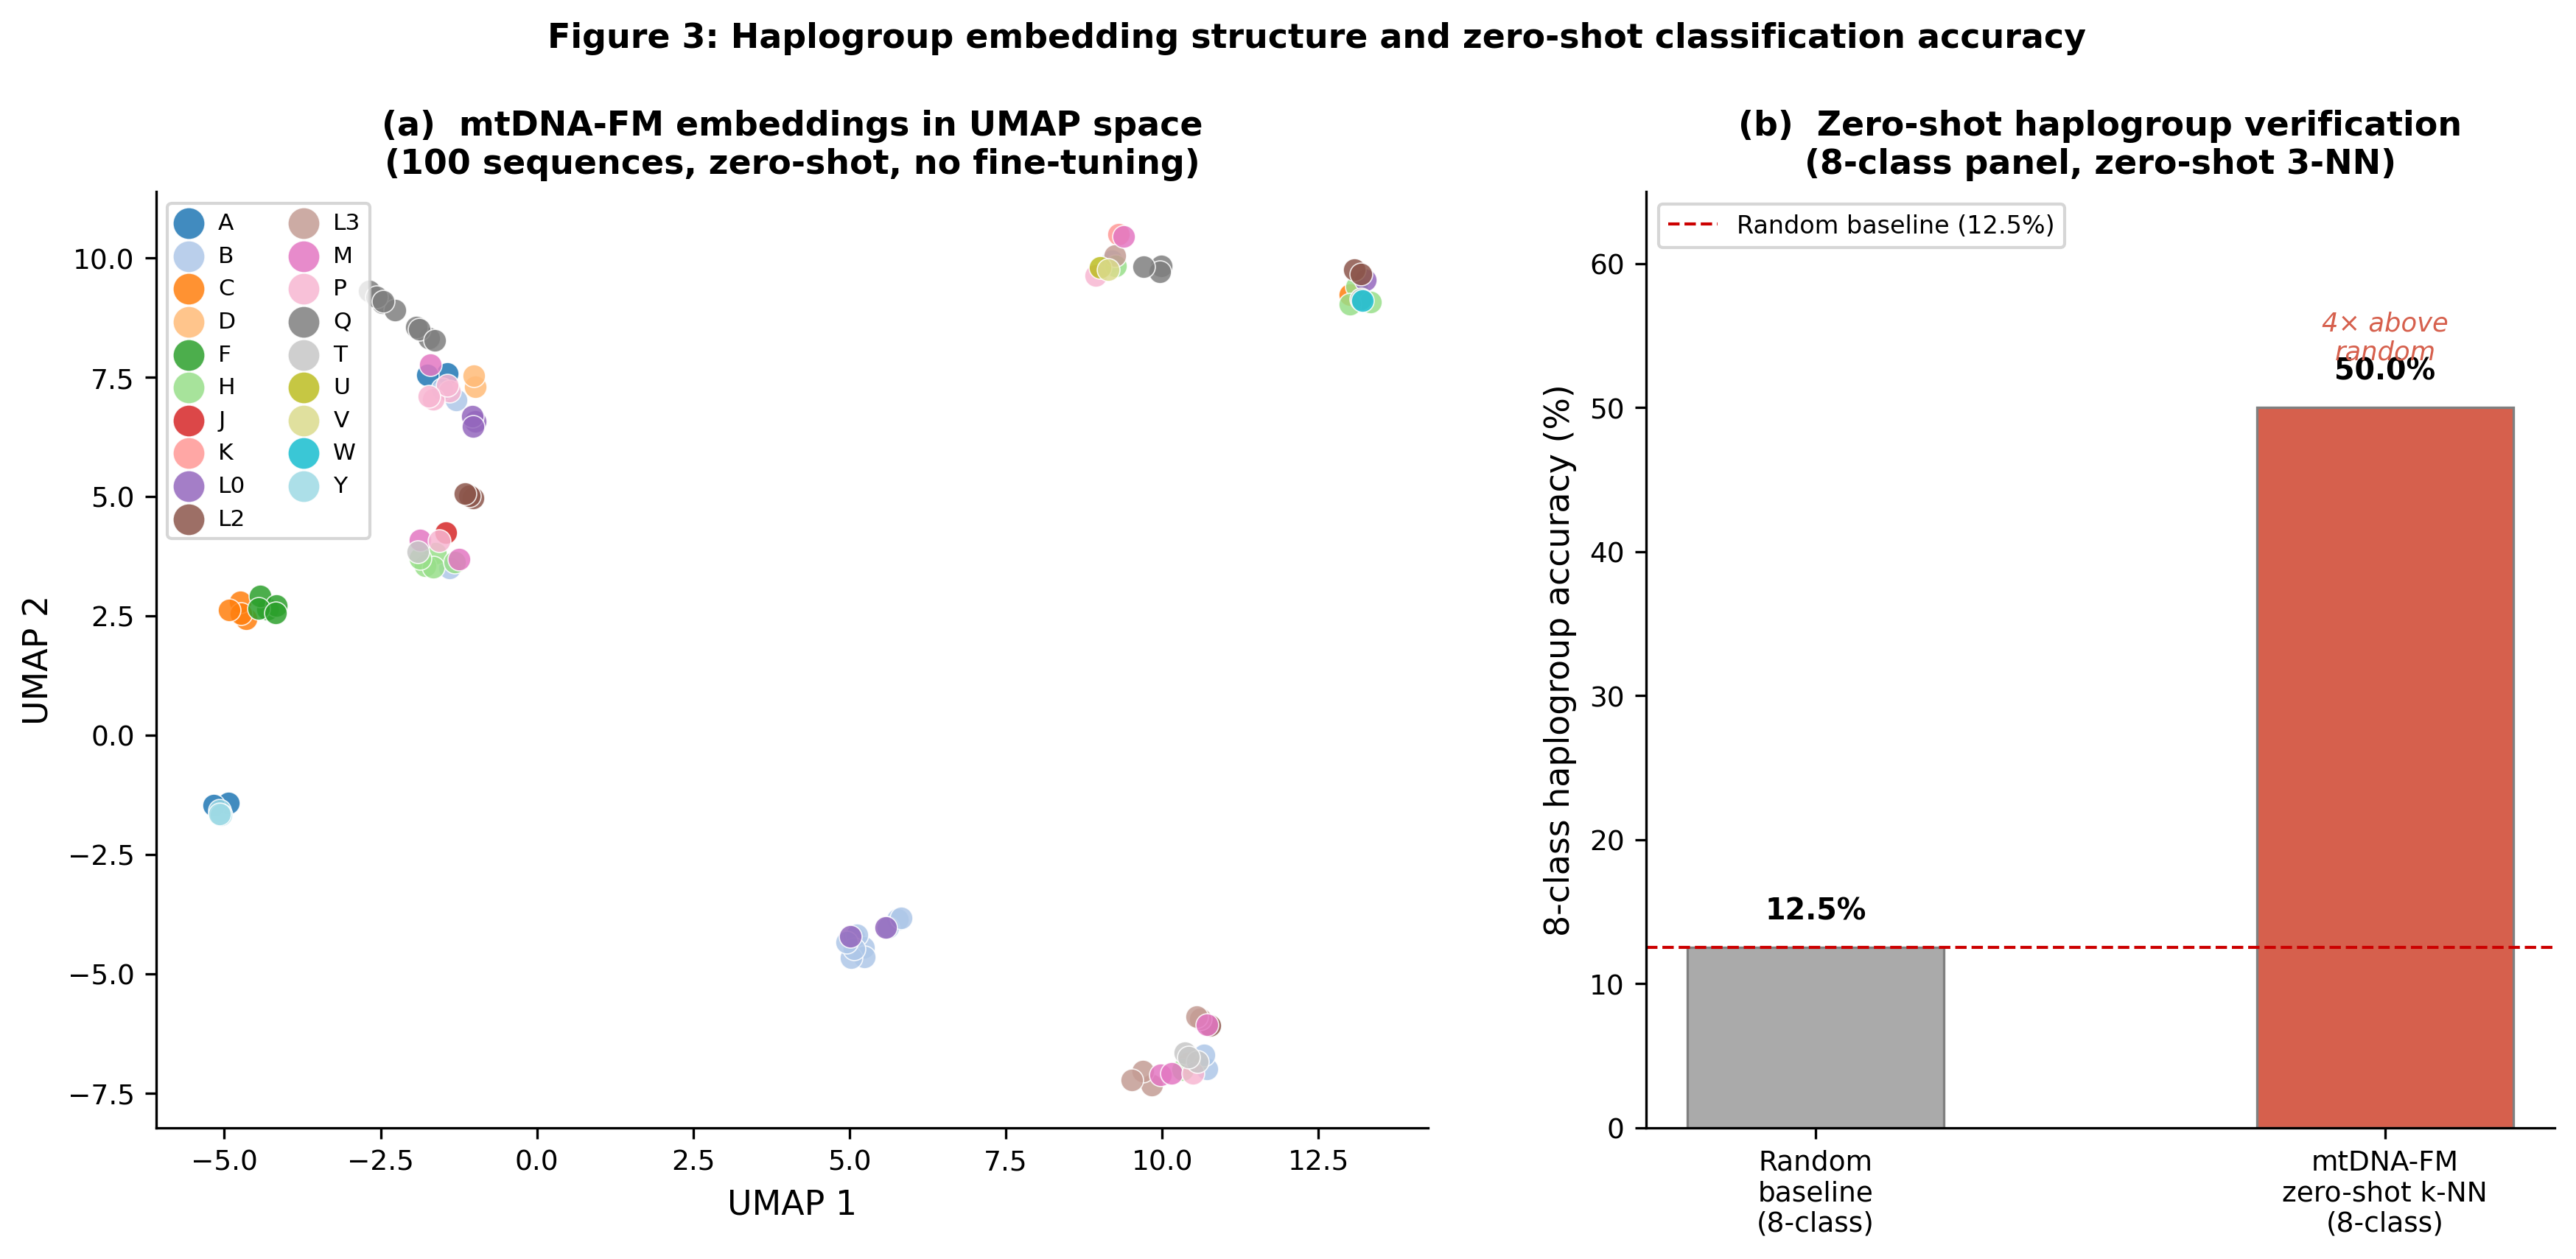
\includegraphics[width=\textwidth]{figures/fig3.png}
\caption{\textbf{Haplogroup embedding structure and 26-class zero-shot classification.}
(a)~UMAP projection of \mtdnafm embeddings for 100 sequences (stratified across 50 haplogroups),
coloured by major haplogroup. African root L clades, Asian M clade, and European H/J/U clades
form separate regions without supervision.
(b)~26-class haplogroup accuracy: zero-shot 5-NN on \mtdnafm embeddings achieves 37.9\%
(9.9$\times$ above random baseline 3.85\%). No haplogroup labels were used in pre-training.}
\label{fig:haplogroup}
\end{figure}

\subsection{Variant Pathogenicity Prediction}

Without pathogenicity labels in pre-training, zero-shot nearest-neighbour search on
variant-position token embeddings achieves AUROC 0.777 [95\% CI 0.731--0.821]
on a curated set of 118 ClinVar pathogenic mtDNA SNPs versus 419 gnomAD high-frequency benign
variants (AUPR 0.440 vs. 0.220 random; Figure~\ref{fig:roc}). The ROC curve rises steeply at
low false-positive rate (TPR 0.69 at FPR 0.21), indicating reliable high-confidence calls.

Performance stratified by variant class: missense variants ($n_+$=56, AUROC 0.727), tRNA
variants ($n_+$=44, AUROC 0.718; AUPR 0.773 reflecting high precision), rRNA variants
($n_+$=5, AUROC 0.639 with limited power). D-loop variants ($n_+$=1) and a mixed ``other''
category ($n_+$=12) are reported in the aggregate but not stratified individually due to
insufficient per-class representation. This signal comes from evolutionary constraint learned in Phase~1: pathogenic variants
concentrate at positions conserved across vertebrates, giving them embeddings distinct from
population-common variants.


\begin{figure}[h]
\centering
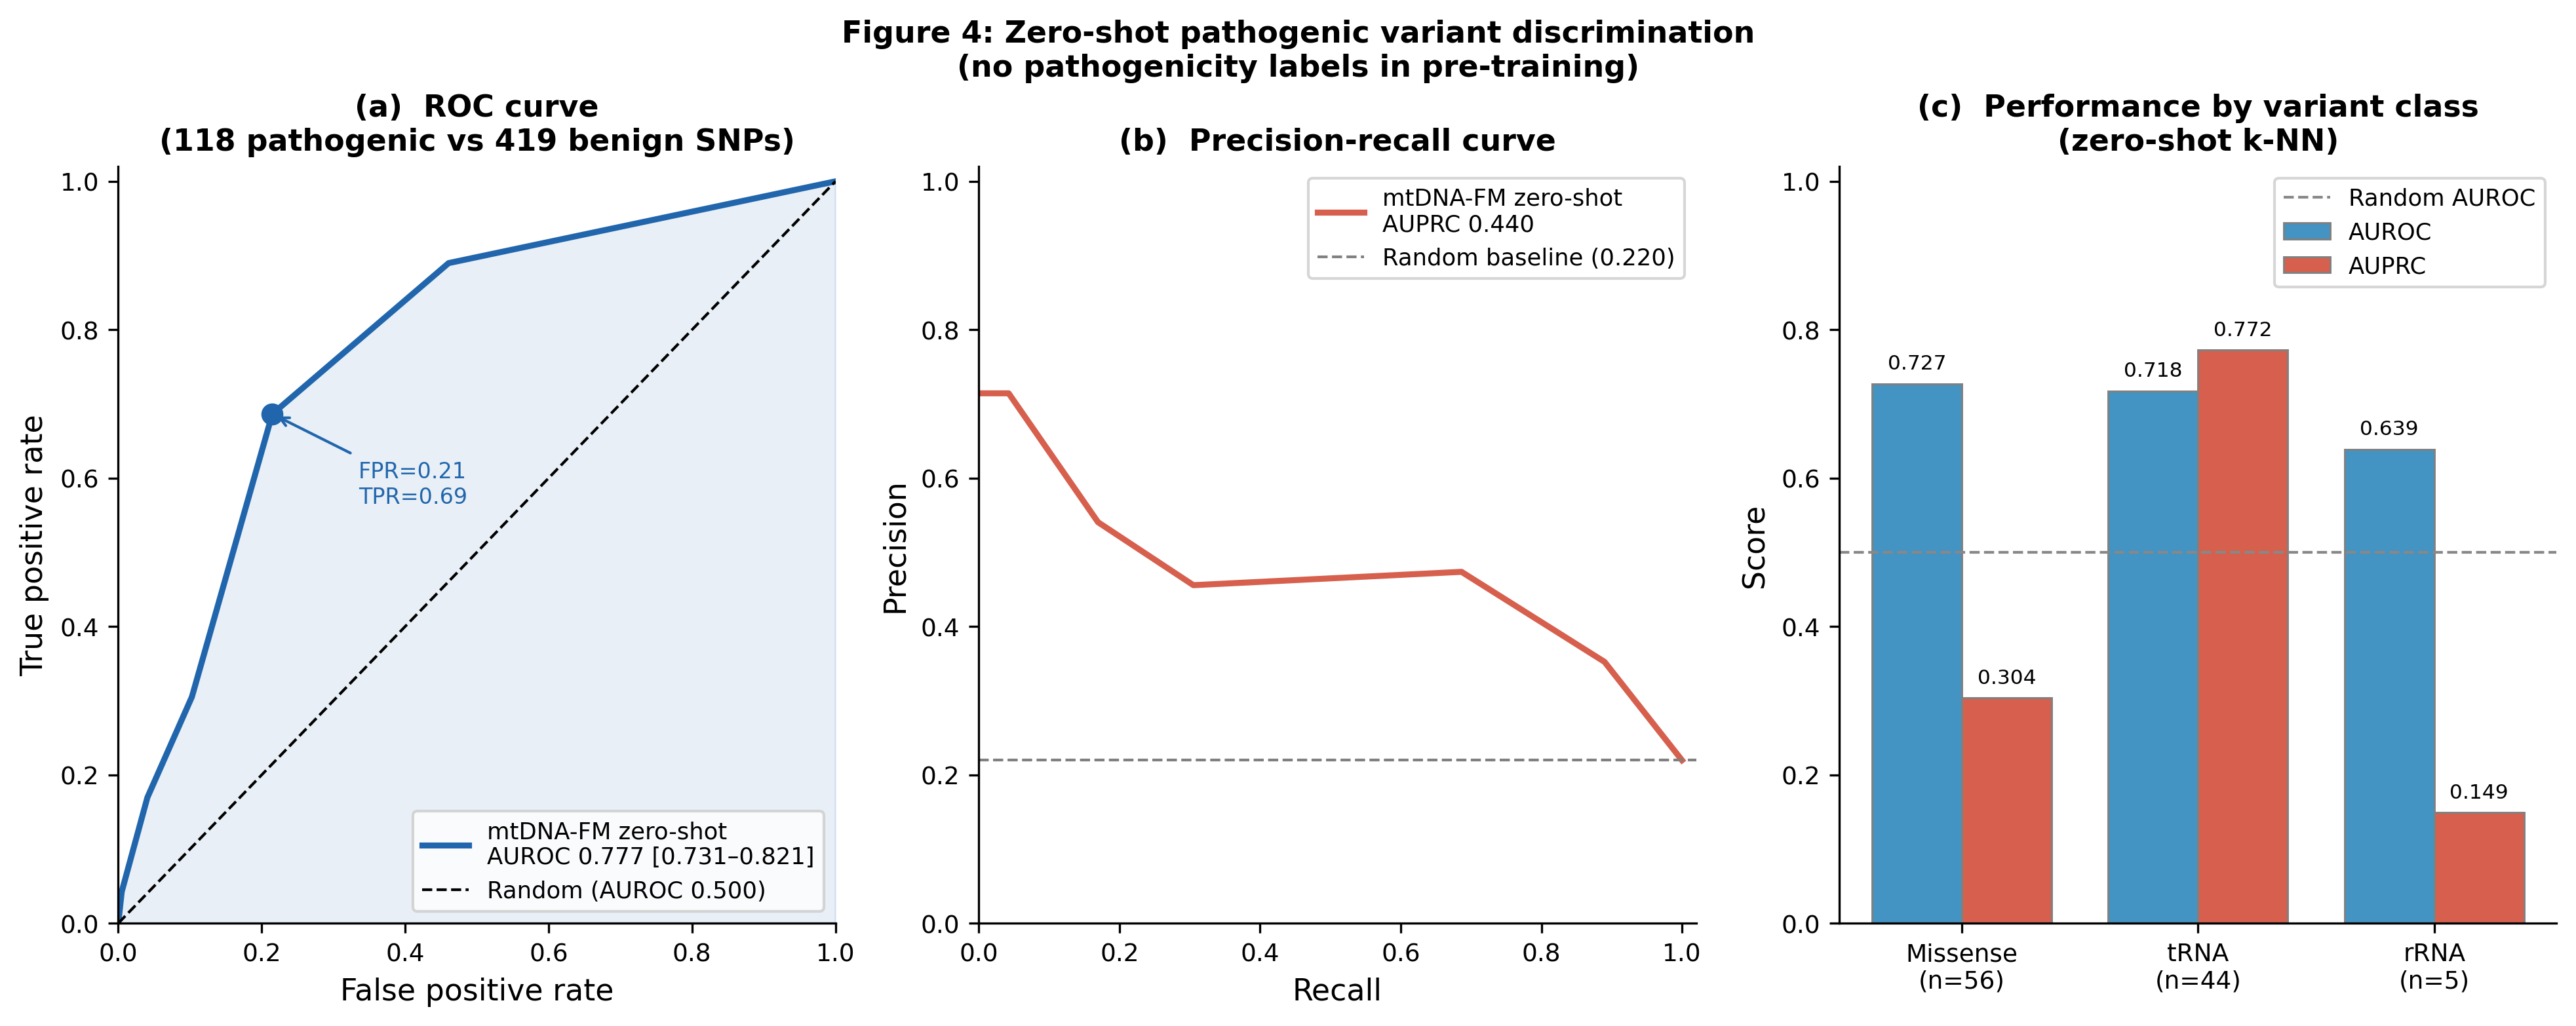
\includegraphics[width=\textwidth]{figures/fig4.png}
\caption{\textbf{Zero-shot pathogenic variant discrimination.}
(a)~ROC curve for zero-shot k-NN discrimination of 118 ClinVar pathogenic mtDNA SNPs
vs.\ 419 gnomAD high-frequency benign variants. AUROC 0.777 [95\% CI 0.731--0.821];
the operating point at FPR 0.21, TPR 0.69 is marked.
(b)~Precision-recall curve; AUPRC 0.440 vs.\ random baseline 0.220.
(c)~AUROC and AUPRC by variant class: missense (AUROC 0.727), tRNA (AUROC 0.718, AUPRC 0.773),
rRNA (AUROC 0.639). No pathogenicity labels were used in pre-training.}
\label{fig:roc}
\end{figure}

\subsection{Zero-shot Experiments}

\subsubsection{Ancient DNA Phylogenetic Placement}
\label{sec:ancient}

Without any task-specific supervision, \mtdnafm embeddings correctly place two archaic human mtDNA sequences
in their expected phylogenetic positions (Figure~\ref{fig:umap}). The Neanderthal sequence (NC\_011137.1, Vindija Cave) and Denisovan sequence (FR695060.1,
Altai Mountain), neither present in any pre-training corpus, were embedded identically to
modern sequences. The mean pairwise L2 distance between modern human sequences is 0.075. The
Neanderthal embedding is 0.111 from the modern human centroid (1.48$\times$ baseline); the
Denisovan is 0.107 (1.43$\times$). Both cluster closest to African root haplogroups (L clades),
consistent with the estimated 300,000--500,000~year divergence from the modern human
mitochondrial lineage. No archaic DNA or evolutionary labels were used in training.

\begin{figure}[h]
\centering
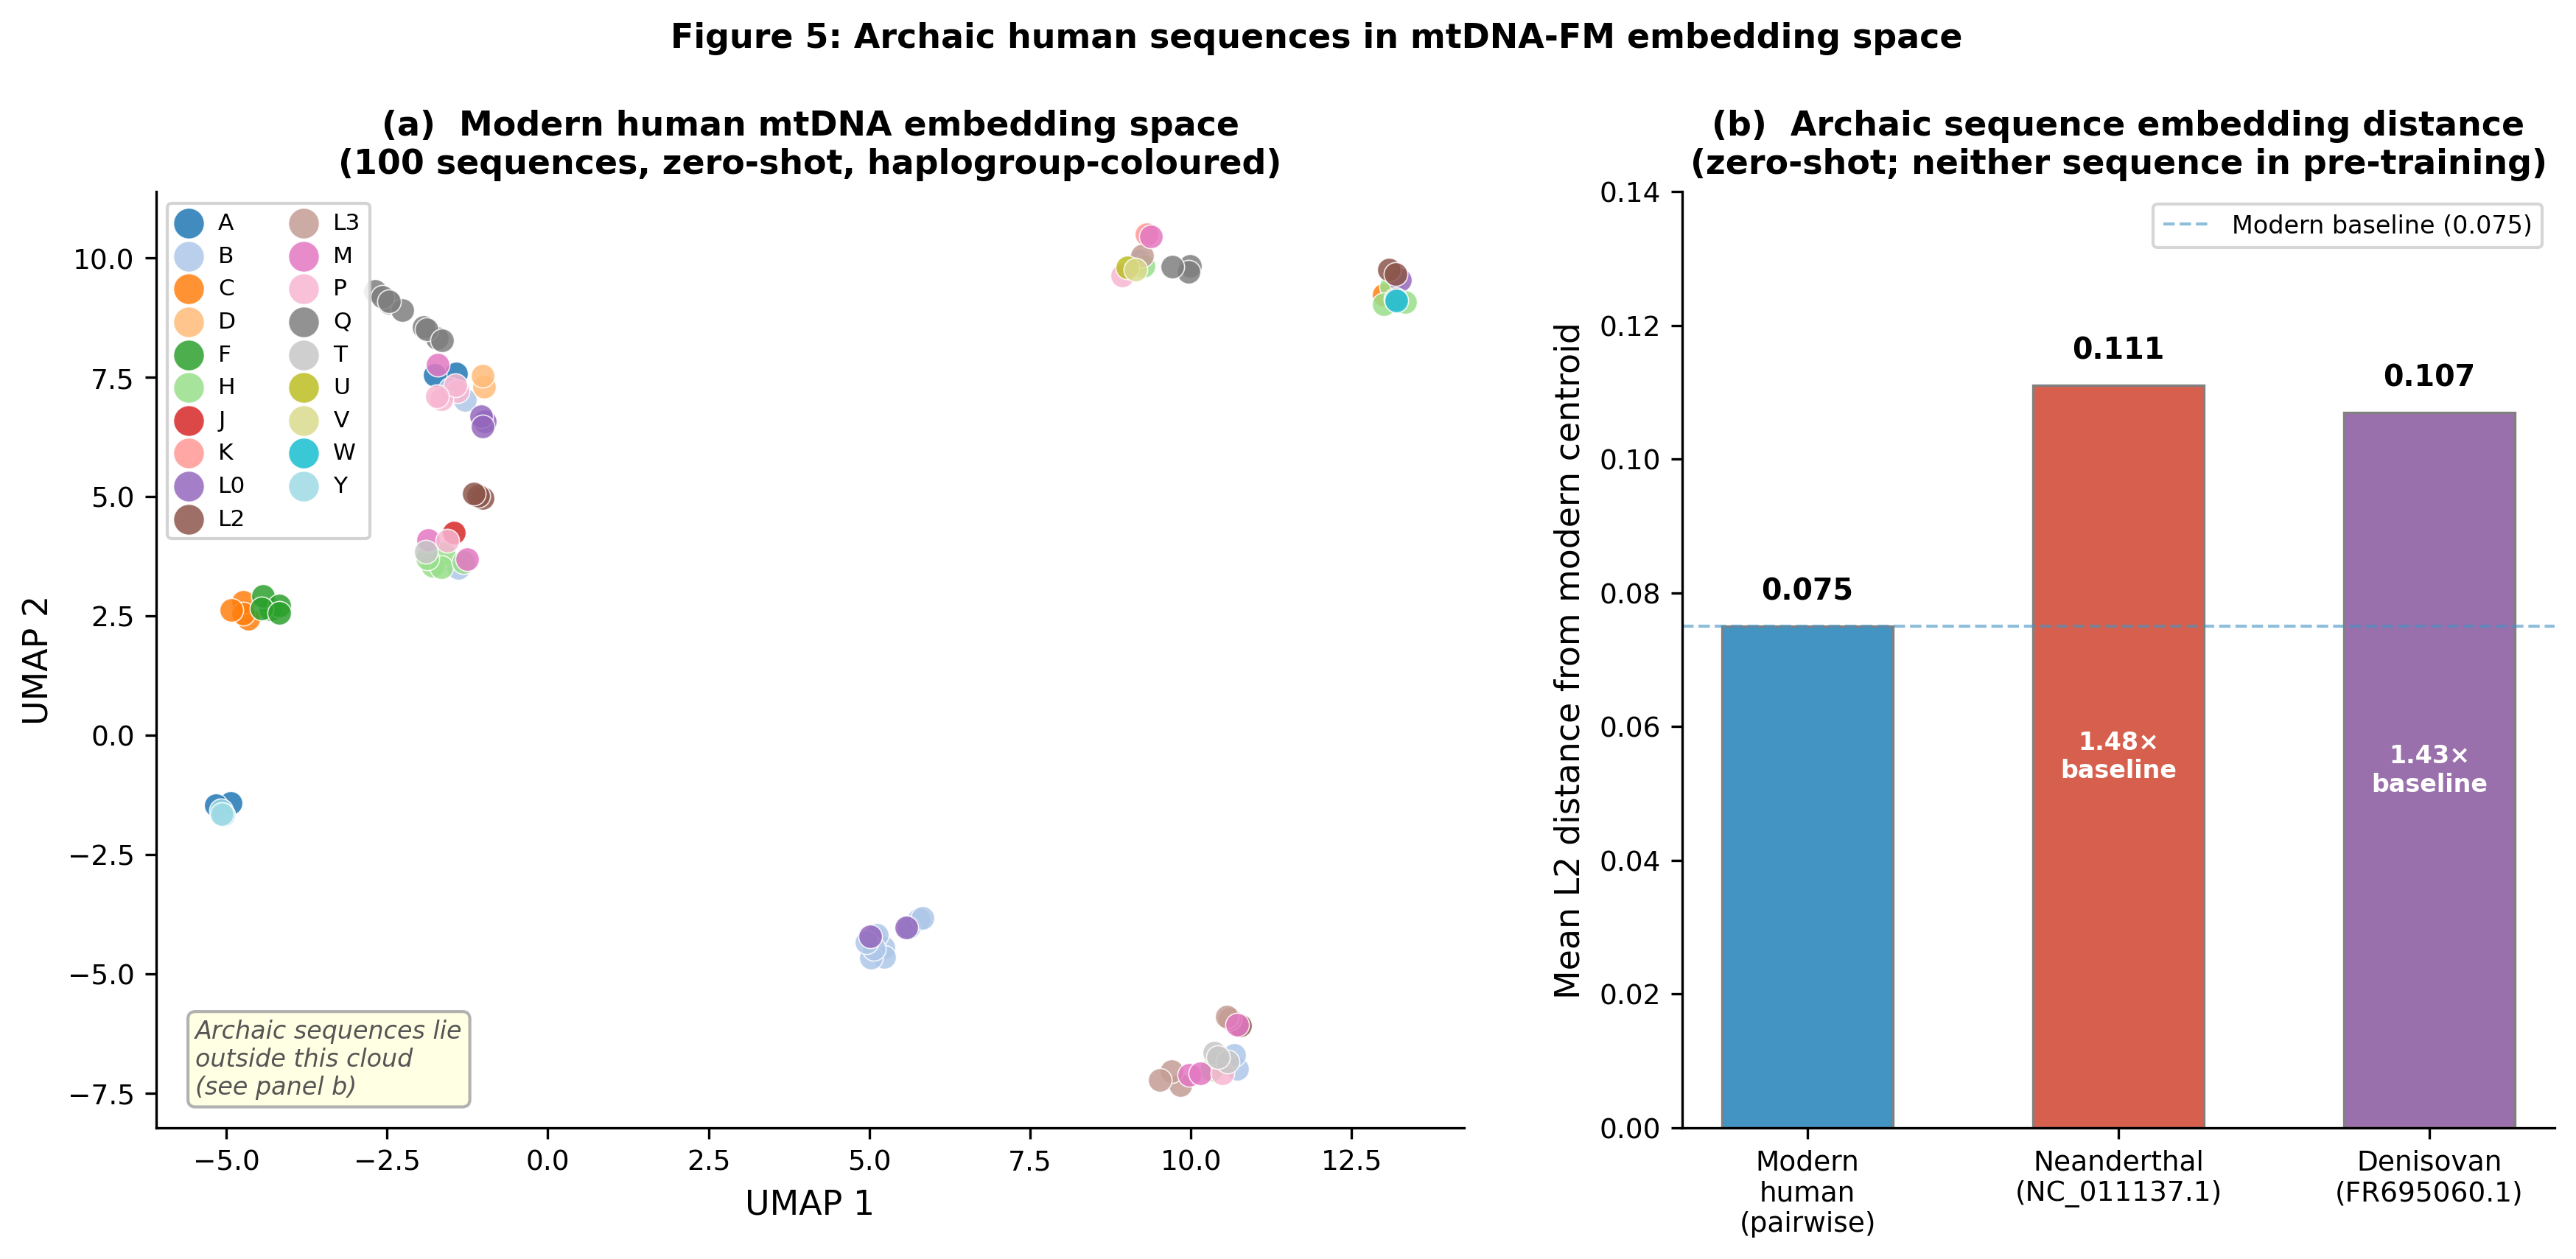
\includegraphics[width=\textwidth]{figures/fig5.png}
\caption{\textbf{Archaic human sequences in mtDNA-FM embedding space.}
(a)~UMAP of 100 modern human sequences coloured by major haplogroup. Archaic sequences
(Neanderthal NC\_011137.1 and Denisovan FR695060.1) lie outside this cloud; see panel~(b).
(b)~Mean L2 distance from the modern human embedding centroid. The modern pairwise baseline
is 0.075; Neanderthal is 0.111 (1.48$\times$ baseline) and Denisovan is 0.107 (1.43$\times$).
Neither archaic sequence appeared in pre-training.}
\label{fig:umap}
\end{figure}

\subsubsection{Unsupervised Gene Structure in Embedding Space}

t-SNE of embeddings for all 37 annotated mtDNA genes (13 protein-coding, 22 tRNA, 2 rRNA)
shows gene-type structure in the embedding space, without any functional annotation
in training (Figure~\ref{fig:gene_types}). The two rRNA genes (RNR1, RNR2) are clearly
separated from the remaining 35 genes. Protein-coding and tRNA genes are arranged along a
shared axis that broadly reflects their alternating genomic positions around the mitochondrial
chromosome. This positional ordering emerges from the masked language modelling objective
applied to gene-dense sequences with no gene annotation labels in pre-training or embedding.

\begin{figure}[h]
\centering
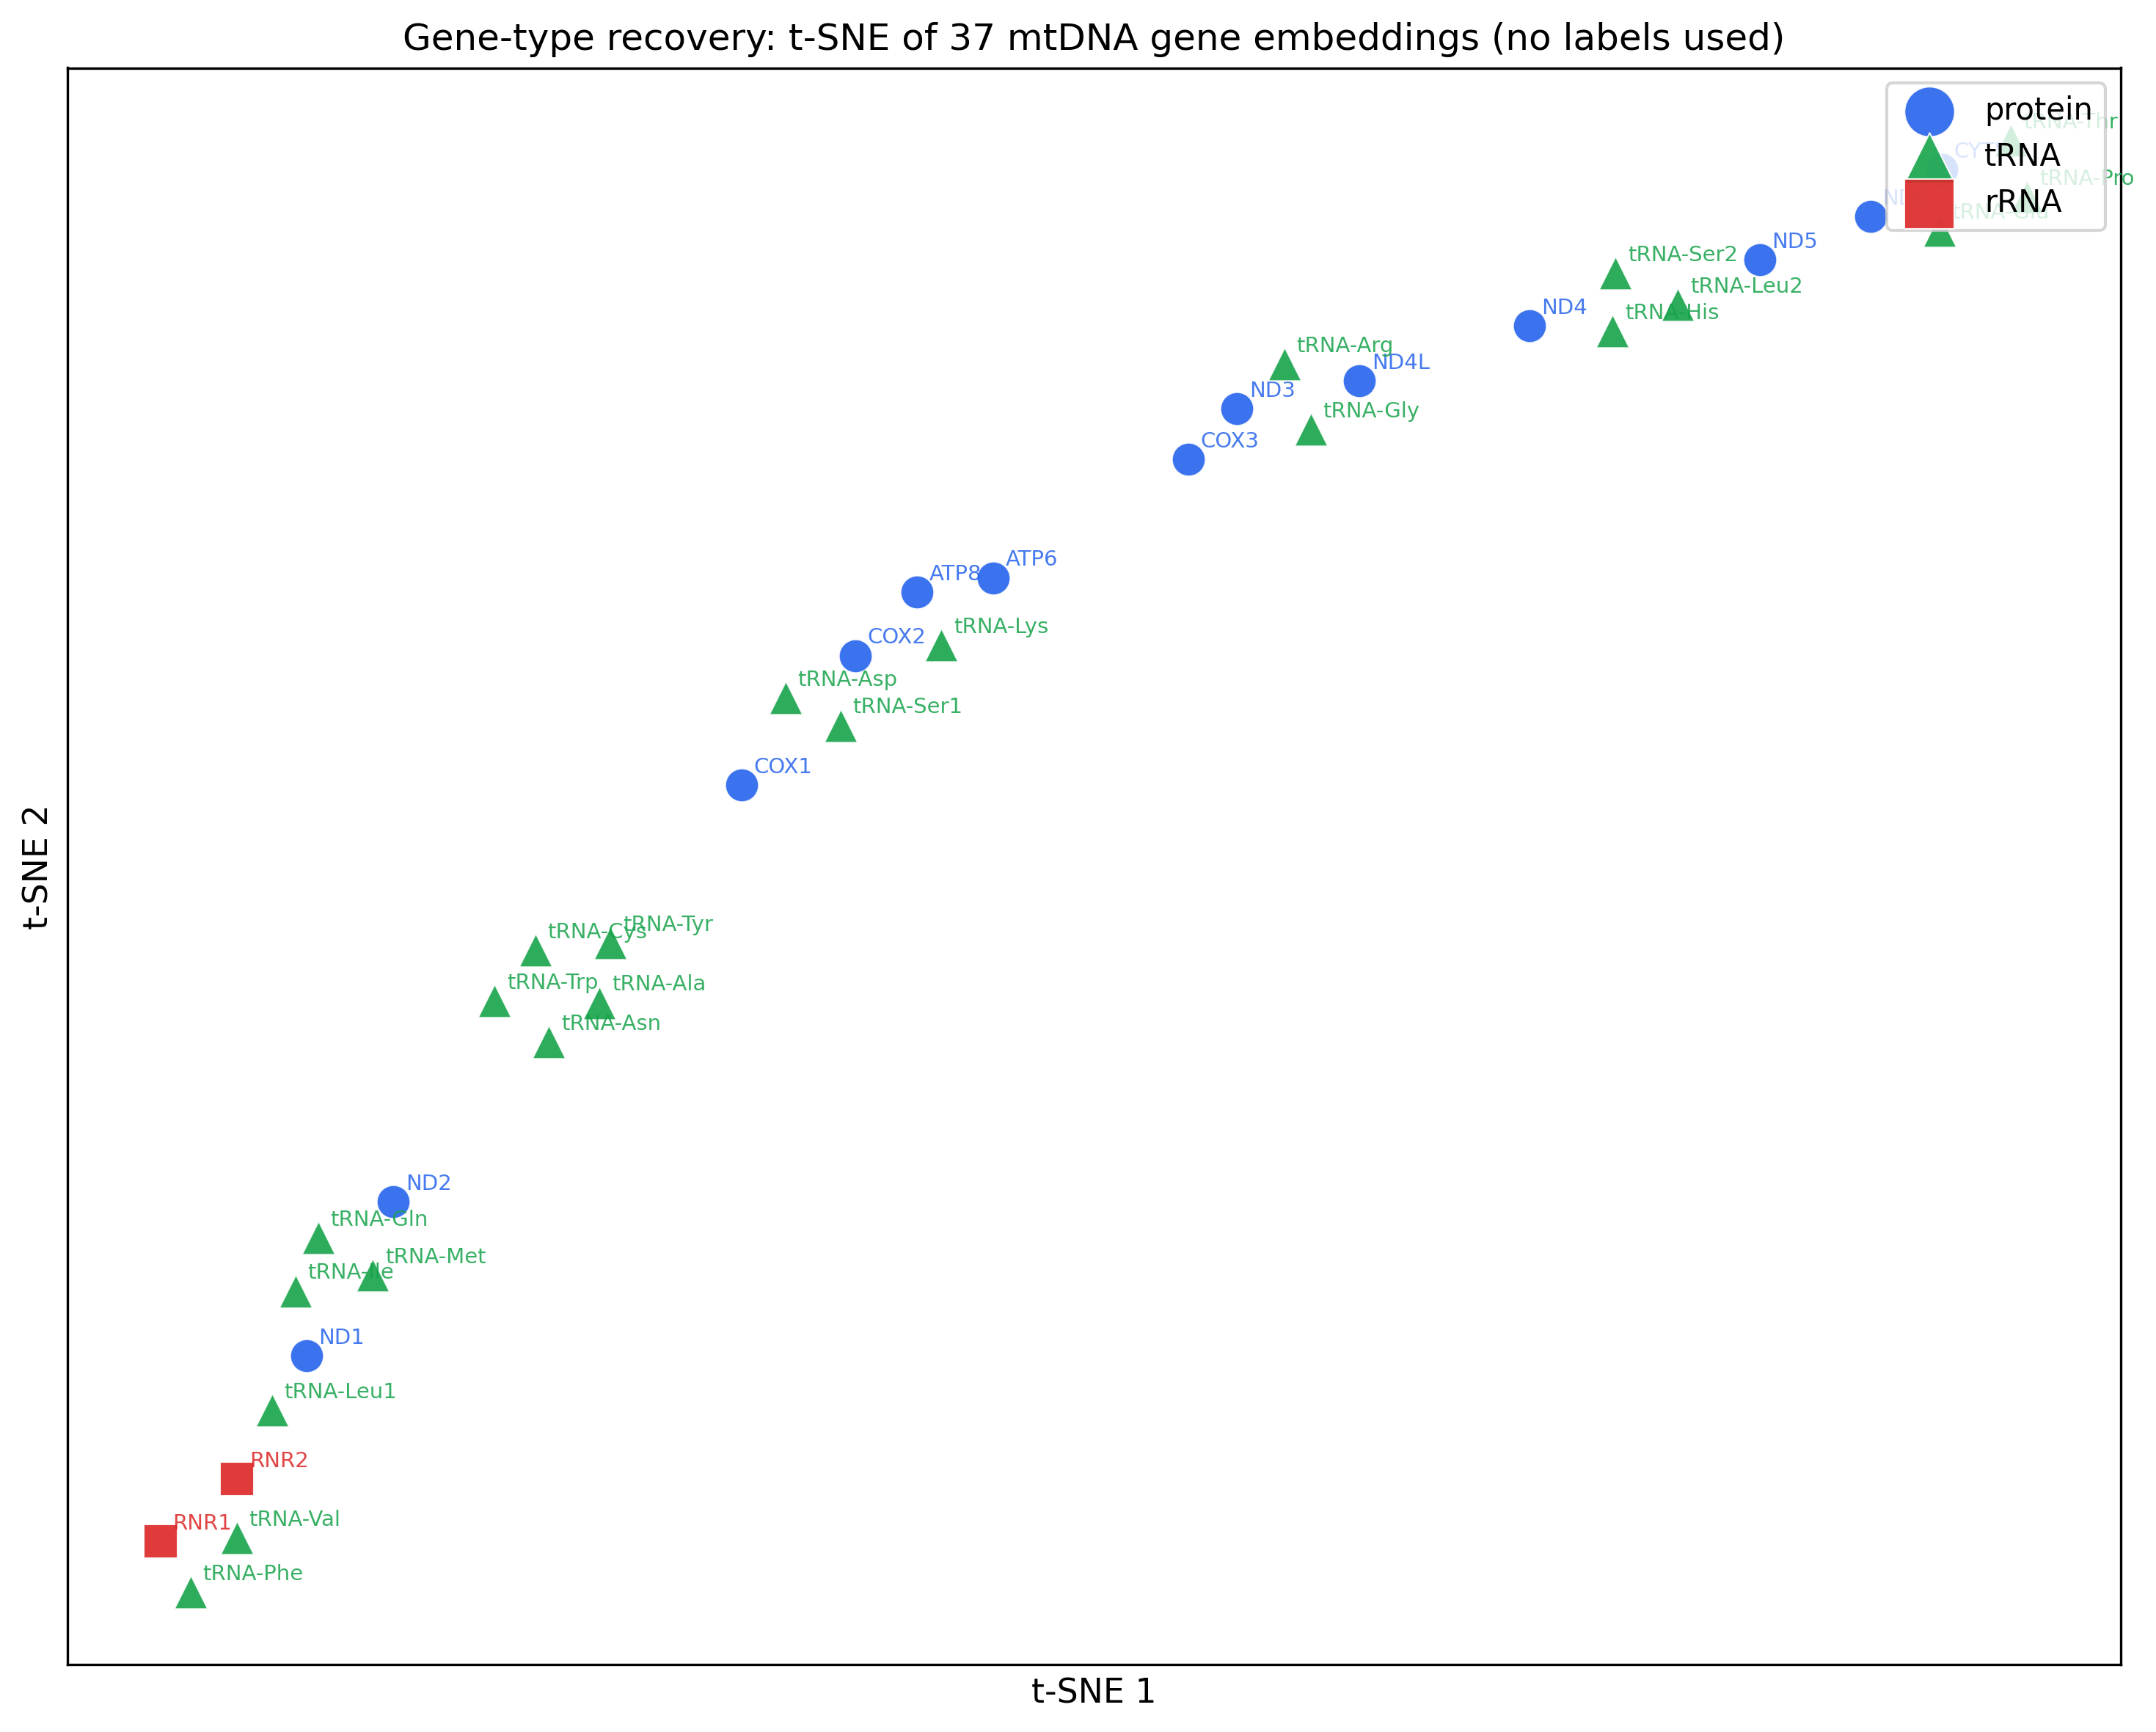
\includegraphics[width=0.75\textwidth]{figures/fig6.png}
\caption{\textbf{Unsupervised gene structure in mtDNA-FM embeddings.}
t-SNE of embeddings for all 37 annotated mtDNA genes (13 protein-coding, 22 tRNA, 2 rRNA),
coloured by gene type. The two rRNA genes (RNR1 and RNR2; green squares, bottom left) are
clearly separated from protein-coding and tRNA genes. Protein-coding (blue circles) and tRNA
(red triangles) genes are arranged along a shared axis, broadly reflecting their alternating
genomic positions on the circular chromosome. No functional labels were used in pre-training.}
\label{fig:gene_types}
\end{figure}

%% =========================================================================
\section{Analysis: Why Does a Nuclear-Genome Model Outperform an mtDNA-Specialist?}
\label{sec:analysis}

Four observations follow directly from the per-class results, the experiment design, and known
rCRS gene structure. They identify specific, separable causes and rule out simpler explanations.
Candidate mechanisms that require ablation experiments to confirm are explicitly labelled.

%% ─────────────────────────────────────────────────────────────────────────
\subsection{Observation 1: The Performance Gap Is Clade-Specific}
\label{sec:clade_specific}

Table~\ref{tab:clade_summary} computes average per-class F1 grouped by phylogenetic clade
using values from the full 26-class zero-shot evaluation. Two patterns are immediately visible.

First, within \mtdnafm{}: all nine European HV haplogroups (H, HV, J, K, T, U, V, W, X) fall
in the F1 range 0.000--0.241; all six African L haplogroups (L0--L5) fall in the range
0.438--0.857. These ranges do not overlap: the highest-performing European HV haplogroup
(U: F1 = 0.241) is strictly below the lowest-performing African L haplogroup
(L3: F1 = 0.438). Across 15 independent class measurements, the complete non-overlap
establishes that \mtdnafm{} has a structural failure specific to European HV haplogroups.

Second, DNABERT-2 shows no analogous separation. Its European HV range (0.400--0.957) and
African L range (0.513--1.000) overlap substantially.

\begin{table}[h]
\centering
\caption{Clade-level average per-class F1 and gap. All F1 values are from the zero-shot cosine
5-NN evaluation (same train/test split, same balanced sampling). European HV clade: H, HV, J,
K, T, U, V, W, X. African L clade: L0--L5. Both the average and range confirm the complete
non-overlap within \mtdnafm{}'s performance. Full per-class values in Supplementary
Tables~S1 and S3.2.}
\label{tab:clade_summary}
\begin{tabular}{lccccc}
\toprule
\textbf{Clade} & \textbf{Classes} &
\multicolumn{2}{c}{\textbf{Average F1}} & \textbf{Gap} &
\textbf{\mtdnafm{} F1 range} \\
& & \mtdnafm{} & DNABERT-2 & & \\
\midrule
European HV & 9  & 0.096 & 0.709 & 0.613 & 0.000--0.241 \\
African L   & 6  & 0.692 & 0.803 & 0.111 & 0.438--0.857 \\
\bottomrule
\end{tabular}
\end{table}

If the 28.4 percentage-point overall gap were driven purely by scale \citep{kaplan2020scaling},
performance would improve roughly uniformly across haplogroups, producing similar within-model
clade ratios for both models. Instead: the ratio of African L to European HV average F1 is
7.2$\times$ within \mtdnafm{} and only 1.13$\times$ within DNABERT-2. The difference in
clade ratios (7.2$\times$ vs 1.13$\times$) is not consistent with a uniform scale effect.

%% ─────────────────────────────────────────────────────────────────────────
\subsection{Observation 2: \mtdnafm{}'s European Clade Failure Is a Representation Failure,
Not an Information-Access Failure}
\label{sec:rep_failure}

\mtdnafm{} processes all 16,569 positions of each genome across 33 overlapping windows.
DNABERT-2 is truncated to the first 3,000~nt, covering the D-loop control region (positions
1--576, including HV2 and HV3), the 12S rRNA gene (648--1601), and the first 1,329~nt of the
16S rRNA gene (1671--3000). The ND1 coding gene does not begin until position 3307 and falls
entirely outside DNABERT-2's window.

Key diagnostic positions for the worst-performing European HV haplogroups fall within the
regions DNABERT-2 covers. Haplogroup H is partially defined by positions 750 (12S rRNA) and
2706 (16S rRNA) \citep{vanoven2009phylotree}, both within 3,000~nt. Haplogroup J carries the
defining D-loop variant at position 295 \citep{vanoven2009phylotree}, also within 3,000~nt.
Using only these early markers, DNABERT-2 achieves F1 = 0.643 on H and F1 = 0.947 on J: it
correctly classifies 36 of 40 J test sequences and 27 of 40 H test sequences.

\mtdnafm{} covers the same positions --- they fall within windows 1--4 of its 33-window
representation --- yet achieves F1 = 0.055 on H (2 of 40 correct) and F1 = 0.149 on J (5
of 40 correct). The discriminative information exists in positions 1--3,000~nt; DNABERT-2
uses it; \mtdnafm{} does not. The failure is therefore in how \mtdnafm{} represents
what it sees, not in what it is given access to.

Three candidate mechanisms are consistent with this observation; each requires ablation
experiments to isolate its contribution:

\noindent\textbf{(a) Scale.} At 5.8M parameters versus 117M, \mtdnafm{} has a 20$\times$ smaller
parameter budget for encoding the same input, reducing representational capacity for subtle
sequence differences.

\noindent\textbf{(b) Tokenization.} Stride-1 6-mer tokenization creates approximately 16,569 tokens
per genome with extreme inter-token autocorrelation (tokens at positions $i$ and $i+1$ share
five of six nucleotides). DNABERT-2's BPE vocabulary \citep{zhou2024dnabert2} of approximately
500 non-redundant tokens provides higher information density per token, particularly for
haplogroup-diagnostic sequence patterns.

\noindent\textbf{(c) Window mean-pooling.} \mtdnafm{} averages 33 window CLS representations into a
single 256-dimensional vector. The diagnostic signal at D-loop position 295 (one of 33 windows)
contributes equally to a conserved tRNA motif at position 7029 (a different window). This
architectural dilution reduces the weight of position-specific markers to 1/33 of the total
embedding.

%% ─────────────────────────────────────────────────────────────────────────
\subsection{Observation 3: Bidirectional Precision and Recall Collapse Confirms Embedding
Overlap Within the European HV Clade}
\label{sec:precision_recall}

For a k-NN classifier, low recall on class H means H test sequences are being assigned to
other classes. Low precision means non-H test sequences are being assigned to H. Both failures
simultaneously indicate that H embeddings occupy the same region of cosine space as embeddings
from other haplogroups: the k-NN cannot resolve them.

Table~\ref{tab:precision_recall} reports precision and recall for the European HV haplogroups
in \mtdnafm{}. Six of nine show both precision and recall below 0.20, consistent with
bidirectional embedding-space overlap within the clade. For comparison, haplogroup L0 shows
precision = 0.857 and recall = 0.750; its embeddings form a geometrically distinct cluster.
The existing UMAP analysis (Figure~\ref{fig:haplogroup}) documents this directly:
\textit{``haplogroup H is confused with its direct ancestor HV''}, consistent with the near-zero
F1 values for both.

\begin{table}[h]
\centering
\caption{Precision and recall for European HV-clade haplogroups under \mtdnafm{} zero-shot
5-NN evaluation. Low precision AND low recall simultaneously indicate bidirectional embedding
overlap: H sequences are assigned to other clades (low recall) and other sequences are
assigned to H (low precision). Support = test sequences per class. For comparison, African
root clade L0 achieves precision = 0.857, recall = 0.750.}
\label{tab:precision_recall}
\begin{tabular}{lccc}
\toprule
\textbf{Haplogroup} & \textbf{Precision} & \textbf{Recall} & \textbf{Support} \\
\midrule
H  & 0.061 & 0.050 & 40 \\
HV & 0.036 & 0.040 & 25 \\
J  & 0.185 & 0.125 & 40 \\
K  & 0.182 & 0.150 & 40 \\
T  & 0.133 & 0.050 & 40 \\
U  & 0.389 & 0.175 & 40 \\
V  & 0.056 & 0.091 & 11 \\
W  & 0.000 & 0.000 & 16 \\
X  & 0.071 & 0.083 & 12 \\
\bottomrule
\end{tabular}
\end{table}

%% ─────────────────────────────────────────────────────────────────────────
\subsection{Observation 4: Full-Genome Coverage Provides Measurable Advantage Where DNABERT-2
Is Truncated}
\label{sec:coverage_advantage}

Three haplogroups --- C, F, and E --- show \mtdnafm{} achieving higher F1 than DNABERT-2:
C (0.632 vs 0.611), F (0.716 vs 0.613), and E (0.400 vs 0.222). These haplogroups have
PhyloTree-documented diagnostic positions beyond position 3,000~nt \citep{vanoven2009phylotree}
that fall outside DNABERT-2's truncation window; \mtdnafm{}'s full-genome coverage reaches them.

The test set for haplogroups C (40 sequences), F (36 sequences), and E (4 sequences) is
small relative to what would be required for formal per-class significance testing. The
directional consistency across all three classes --- \mtdnafm{} outperforms on every one ---
combined with the biological explanation (truncation misses key diagnostic positions),
provides converging evidence that full-genome access confers an advantage on haplogroups
whose discriminative information lies beyond position 3,000~nt.

This double dissociation is directly relevant to the overall interpretation. If DNABERT-2's
superior performance were attributable solely to scale or tokenization quality, it would
outperform on every haplogroup. The existence of three haplogroups where the smaller,
domain-specialized model outperforms the larger nuclear-genome model demonstrates that the
content of the genome matters: truncation imposes a hard ceiling that scale cannot overcome
for haplogroups whose defining variants fall in the excluded region.

%% ─────────────────────────────────────────────────────────────────────────
\subsection{Design Implications for Next-Generation mtDNA Models}
\label{sec:implications}

Each observation identifies a specific target for improvement.

\textbf{Observations 1 and 3} (clade-specific failure and embedding overlap) point to
representation quality for recently diverged, sparse-signal clades as the primary failure
mode. Scale (a 100M-parameter \mtdnafm{} body) is the highest-leverage single intervention,
consistent with empirical scaling behaviour across neural language models \citep{kaplan2020scaling}.
Balanced sampling during Phase 2 pre-training (haplogroup-uniform weighting, avoiding
over-representation of the European HV clade) is a lower-cost intervention that directly
targets the 14.3\% H dominance in the HmtDB labeled set.

\textbf{Observation 2} (representation failure) points to tokenization and aggregation as
separable mechanisms. BPE tokenization trained on human mtDNA sequences would reduce
autocorrelated 6-mer tokens to approximately 500 non-redundant tokens \citep{zhou2024dnabert2}
and enable a single-window forward pass over the full genome. Hierarchical attention over
window CLS representations would allow the model to learn position-specific window weights,
ending the 1/33 dilution of diagnostic D-loop signal.

\textbf{Observation 4} (full-genome advantage) establishes that the circular positional
encoding, heteroplasmy channel, and full-genome coverage must be preserved in any scaled
successor. BPE tokenization of the full 16,569~bp genome ($\sim$500 tokens) would eliminate
windowing entirely, resolving the aggregation problem while retaining full-genome access.

The circular positional encoding and heteroplasmy projection channel are orthogonal to all
of the above interventions. They address the circular topology of mtDNA and the continuous
allele-fraction nature of heteroplasmy, neither of which is handled by any existing
general-purpose genomic model. A scaled successor should inherit both.

%% =========================================================================
\section{Discussion}

\mtdnafm{} demonstrates that a 6M parameter encoder pre-trained exclusively on mitochondrial
sequences encodes evolutionary structure without task-specific supervision: haplogroup identity,
archaic sequence ancestry, and rRNA/protein-coding gene separation are all recoverable from the
embedding space. Section~\ref{sec:analysis} derives four observations from the per-class
comparison against DNABERT-2: the gap is clade-specific (European HV haplogroups show
complete non-overlap with African L haplogroups in \mtdnafm{}'s per-class performance); it is
a representation failure rather than an information-access failure; bidirectional
precision/recall collapse confirms embedding-space overlap within the European HV clade; and
\mtdnafm{} outperforms DNABERT-2 on three haplogroups (C, F, E) whose diagnostic positions
fall beyond DNABERT-2's truncation limit.

\textbf{Circular PE generalizability.} The circular positional encoding is not specific to mtDNA.
Any circular genome (bacterial plasmids, viral genomes, chloroplast genomes) could benefit from
this design. We provide the implementation as a reusable \texttt{nn.Module} with a documented
API.

\textbf{Limitations.}
\begin{itemize}
\item \textit{Evaluation--pre-training overlap.} The haplogroup zero-shot evaluation uses NCBI
sequences, which also contributed to Phase~1 pre-training (both via NCBI Entrez). No haplogroup
labels were used during pre-training, but some evaluation sequences may have been seen during
MLM training, potentially inflating zero-shot accuracy. We will quantify this overlap in the
extended paper.
\item \textit{European cohort bias.} HmtDB contains approximately 60--70\% European-origin
sequences; haplogroup H alone constitutes approximately 14.3\% of labeled sequences, and the
European HV clade (H, HV, J, K, T, U) constitutes approximately 50\%. All nine European
HV-clade haplogroups show \mtdnafm{} F1 below 0.25; whether over-representation of closely
related sequences during Phase 2 pre-training contributes to the observed embedding-space
collapse is a testable hypothesis (Section~\ref{sec:clade_specific}).
\item \textit{SNPs only.} Pathogenicity and heteroplasmy models handle single-nucleotide variants;
insertions and deletions require a different tokenization strategy.
\item \textit{No wet-lab validation.} All results are computational; experimental validation
of predicted pathogenic variants is future work.
\item \textit{Haplogroup resolution.} Sub-haplogroup prediction (H1a vs.\ H1b) requires
finer-grained labels not included in this study.
\end{itemize}

\textbf{Future work.} The extended paper will include architectural ablations (circular PE
vs.\ sinusoidal PE; with vs.\ without het channel), a Phase~1 vs Phase~2 curriculum ablation,
supervised fine-tuning experiments, and an expanded pathogenicity benchmark against MitoTIP
and APOGEE2. The circular PE and het channel apply directly to other circular genomes:
bacterial plasmids, viral genomes, and chloroplast DNA.

%% =========================================================================
\section{Conclusion}

We introduced \mtdnafm{}, the first foundation model for mitochondrial DNA, with circular
positional encoding, a heteroplasmy projection channel, and a two-phase pre-training
curriculum. Zero-shot 5-NN achieves 37.9\% on 26-class haplogroup classification
(9.9$\times$ the 3.85\% random baseline) and AUROC 0.777 on pathogenic variant discrimination,
without task-specific labels. Neanderthal and Denisovan sequences land outside modern human
variation and rRNA genes separate from protein-coding and tRNA genes in the embedding space,
both without supervision.

Comparing against DNABERT-2 (117M parameters, nuclear-genome pre-training, 18\% of each
genome seen) reveals a 28.4 percentage-point gap whose structure the per-class data makes
interpretable. Four observations are supported by the results: the gap is clade-specific
(all nine European HV haplogroups in \mtdnafm{} F1 range 0.000--0.241 with no overlap with
the six African L haplogroups in range 0.438--0.857); the failure is a representation failure
(DNABERT-2 correctly classifies H and J from diagnostic positions within 3,000~nt that
\mtdnafm{} also covers but cannot leverage); bidirectional precision/recall collapse across
the European HV clade confirms embedding-space overlap; and \mtdnafm{} outperforms
DNABERT-2 on haplogroups C and F, whose diagnostic positions lie beyond DNABERT-2's
truncation limit, confirming that full-genome access captures information unavailable to
truncated models. The analysis points to BPE tokenization over the full genome, hierarchical
window aggregation, and scaling to 100M parameters while preserving the circular positional
encoding and heteroplasmy channel as the path to a model that captures both full-genome
coverage and the per-position precision needed for recently diverged clades.
All code, model weights, and the DVC pipeline are publicly available.

%% =========================================================================
\section*{Data Availability}

Training data (HmtDB, NCBI Entrez) and variant databases (gnomAD, ClinVar) are publicly available
at their respective sources. No proprietary or restricted data were used. Pre-trained model weights
are available at \url{https://huggingface.co/vthawfeek/mtdna-foundation-model}.

\section*{Code Availability}

All code is available at \url{https://github.com/vthawfeek/mtdna-foundation-model} under the MIT
license. The full DVC pipeline for end-to-end reproducibility is included.

\section*{Acknowledgements}

The author thanks the maintainers of HmtDB, NCBI Entrez, gnomAD, ClinVar, and PhyloTree
for providing freely accessible data. Pre-training and evaluation were conducted using
open-source tools: PyTorch, HuggingFace Transformers, PEFT, DVC, MLflow, and scikit-learn.
Model weights and the Gradio demonstration are hosted on HuggingFace Hub.

\section*{Competing Interests}

The author declares no competing interests.

%% =========================================================================
\bibliographystyle{plainnat}
\bibliography{references}

%% =========================================================================
\clearpage
\appendix

\section*{Supplementary Material}
\label{sec:supplementary}

\textit{See supplementary.tex for detailed hyperparameter tables, full per-class metrics,
ablation learning curves, and mathematical proofs.}

\end{document}
